\chapter{A proof-of-concept method to identify enhancers using constraints on binding site motifs}
\label{chap:Proof of concept method to identify enhancers}

%%%%%%%%%%%%%%%%%%%%%%%%%%%%%%%%%%%%%%%%%%%%%%%%%%%%%%%%%%%%%%%%%%%%%%%%%%%%%%%%
\section{Introduction}
%%%%%%%%%%%%%%%%%%%%%%%%%%%%%%%%%%%%%%%%%%%%%%%%%%%%%%%%%%%%%%%%%%%%%%%%%%%%%%%%

Enhancers are non-coding elements of the human genome that act as switches to regulate when and where genes are expressed. This feature of enhancers thus makes them a key contributor to tissue-specific gene expression during tightly controlled processes such as development and homeostasis \cite{levine2010,heinz2010,small1992,spitz2012,liu2012a,swanson2010a}. Most disease mutations are located within enhancers. Additionally, the interplay between the syntax-the order, orientation, and spacing of transcription factor binding sites (TFBSs)-and binding affinity can finely control gene expression patterns through a mechanism known as "enhancer grammar" \cite{maurano2012,tak2015a,visel2009,jindal2021}. However, there is still a lack of understanding of how the grammar of a particular genomic sequence relates to proper or improper enhancer function \cite{jindal2021}. With the increasing volume of genomic data collected due to next-generation sequencing (NGS), it is necessary to develop computational tools to mine genomes to pinpoint tissue-specific enhancers for further study \cite{leonelli2019,marx2013,pal2020,stephens2015}. 

Computational tools to identify enhancers have primarily focused on chromatin signatures \cite{meuleman2020,zinzen2009}. While tissue-specific epigenomic data can sometimes pinpoint tissue-specific enhancers, this approach largely ignores the possible link between TFBS organization, or enhancer grammar, and tissue-specific activity \cite{jindal2021,grossman2017,ryan2020,king2020a,halfon2019}. Currently, four different models for enhancer-TFBS interactions have been proposed. The billboard model suggests that there are no constraints on TFBS arrangements within an enhancer—only that TFBSs be present somewhere in the sequence \cite{liu2012a,kulkarni2003,jindal2021}. In contrast, the enhanceosome model suggests that TFBSs must reside in a precise arrangement within an enhancer \cite{bazett-jones1994,thanos1995,panne2007,melnikov2012,jindal2021}. The TF-collective model suggests that in the absence of TFBS organization within an enhancer sequence, there is collective occupancy of the enhancer sequence by transcription factors (TF) through a combination of direct TF binding to TFBSs and TF-TF interactions \cite{junion2012,jindal2021}. There is a new model that has been proposed by our group that encompasses the previous three models as a spectrum based on the interplay of constraints. We call this "dependency grammar." Dependency grammar proposes that the interplay between TFBS syntax and affinity is shaped by biological, mechanistic, and evolutionary constraints \cite{jindal2021}. Thus, identifying TFBSs within putative enhancers is a critical first step in determining enhancer grammar. 

In a previous study, we tested 90 genomic regions containing Zic and ETS TFBSs and found additional binding sites-Brachyury (Bra) and FoxA-that may be playing a role in dictating enhancer activity in the \textit{Ciona} notochord. From the nine sequences we found to be active, we created three groupings based on what collection of Zic, ETS, Bra, and FoxA binding sites were present: (1) Zic and ETS; (2) Zic, ETS, and Bra; and (3) Zic, ETS, Bra, and FoxA (Chapter \ref{chap:Diverse logics encode notochord enhancers}) \cite{song2022}. Interestingly, when testing genomic regions from the organism \textit{Ciona intestinalis type A} (\textit{Ciona}) containing these sites, we came to the striking conclusion that clusters of binding sites alone are not sufficient to drive expression even though all the transcription factors at play have some biological association with the nervous system or notochord (Chapter \ref{chap:Diverse logics encode notochord enhancers}) \cite{song2022}. Here, we focus on laying the groundwork for expanding the scope of the previous study to understand how enhancers regulated by Zic and ETS encode notochord expression within \textit{Ciona} using an updated genomic reference sequence developed after we performed our initial screen by Satou \textit{et al.} (2019) \cite{satou2019}. We then apply our methods to perform large searches for clusters of motifs within other vertebrate genomes, including chicken, mouse, zebrafish, and human. We have also developed EnGAGE (\textbf{E}ntire \textbf{G}enome se\textbf{A}rches for \textbf{G}rammars of \textbf{E}nhancers), a proof-of-concept computational framework to search for tissue-specific enhancers within genomes using one's knowledge of TFBS motif signatures. We propose that in the future, this tool can be further developed to look for enhancer grammar by allowing users to add constraints on TFBS syntax or affinity. In the following, we demonstrate the potential future synergy between EnGAGE and massively parallel reporter assays (MPRAs) to study the \textit{Ciona} notochord enhancers. 

%%%%%%%%%%%%%%%%%%%%%%%%%%%%%%%%%%%%%%%%%%%%%%%%%%%%%%%%%%%%%%%%%%%%%%%%%%%%%%%%
\section{Results}
%%%%%%%%%%%%%%%%%%%%%%%%%%%%%%%%%%%%%%%%%%%%%%%%%%%%%%%%%%%%%%%%%%%%%%%%%%%%%%%%

\subsection{Searching for clusters of Zic and ETS sites within an updated \textit{Ciona} genome}

In our previous study, we identified regions across the \textit{Ciona} genome containing one Zic site and at least two ETS sites within 30 bp of the Zic site (Chapter \ref{chap:Diverse logics encode notochord enhancers}) \cite{song2022,farley2016}. Within the study, we selected 90 of these identified regions to comprise the "ZEE Library." While we were able to identify a suitable number of ZEE elements to perform an enhancer screen, there were two key limitations in our initial search methodology that we wanted to address in an updated search. The first limitation was the genomic reference used for \textit{Ciona}. While completing the analyses for our previous study, a new genomic reference for \textit{Ciona} was released using more modern next-generation sequencing methods in 2019—the previous genome reference was assembled in 2008 \cite{satou2019,dehal2002}. The second limitation of our previous search was the inherent search design itself. Because we fixed the Zic site in the center of the genomic element, we potentially missed functional ZEE elements that did not follow this constraint. To continue studying the notochord dependency grammar we previously identified at a greater scale, we developed a new search methodology that improved upon these limitations. We improved our methods by using the updated \textit{Ciona} genomic reference and allowing for more flexibility in binding site location when searching for regions of interest containing Zic and ETS. 

For the next iteration of our search, we identified 100 bp regions in the updated \textit{Ciona} genome containing at least one Zic site and at least two non-overlapping ETS sites. Like our previous approach, we searched for ETS sites using the core motif, \verb|GGAW| (\verb|GGAA| or \verb|GGAT|), to consider all ETS sites regardless of affinity \cite{lamber2008,wei2010,song2022}. We also defined Zic sites using EMSA and enhancer mutagenesis data from previous studies \cite{matsumoto2007a,takahashi1999,yagi2004,song2022}. Using this approach, we identified 4,434 regions with at least one Zic and two ETS sites. Within this study, we define these regions as KYN elements to reference the new “KY” \textit{Ciona} genome assembly, and we are looking at “N,” or notochord, enhancers. In our previous study, we found that two other transcription factors expressed in the notochord, Bra and FoxA, may also contribute to the activity of some enhancers that rely on Zic and ETS. Therefore, we also searched the updated KYN library for these other TFBSs (Chapter \ref{chap:Diverse logics encode notochord enhancers}) \cite{song2022}. Thus, we have three groupings of TFBSs that we were interested in: (1) Zic and ETS, (2) Zic, ETS, and Brachyury (Bra), and (3) Zic, ETS, Bra, and FoxA. In associating our KYN elements with each of these groups, we found that 65.9\% belonged to the Zic/ETS group (2,863/4,344 KYN elements), 31.9\% belonged to the Zic/ETS/FoxA group (1,384/4,344 KYN elements), and 4.3\% belonged to the Zic/ETS/FoxA/Bra group (187 KYN elements) (Figure ~\ref{fig:2 zee library}A). 

After determining our genomic elements of interest, we wanted to evaluate how many ZEE elements (see \ref{chap:Diverse logics encode notochord enhancers}) exist within the new KYN library using Magic-BLAST \cite{boratyn2019}. We created a custom BLAST database using the KYN elements as a reference, then searched for our ZEE elements within this custom database. Of the ZEE elements included in our previous study, 76.7\% were present (69/90 ZEE elements) in our new KYN elements (Figure \ref{fig:1 zee comparison}). Additionally, 77.8\% of the ZEE elements expressed in the notochord were present in the KYN library (7/9 ZEE notochord-expressing elements), including the Brachyury Shadow (BraS) enhancer and the LAMA1/3/5 and LRIG1/2/3 enhancers, which our studies have previously identified (Figure \ref{fig:1 zee comparison}). Additionally, one element, ZEE86, matched two KYN elements—KYN2713 and KYN4077 (Figure \ref{fig:1 zee comparison}). 

\begin{landscape}
    \begin{figure}[h]
        \centering
        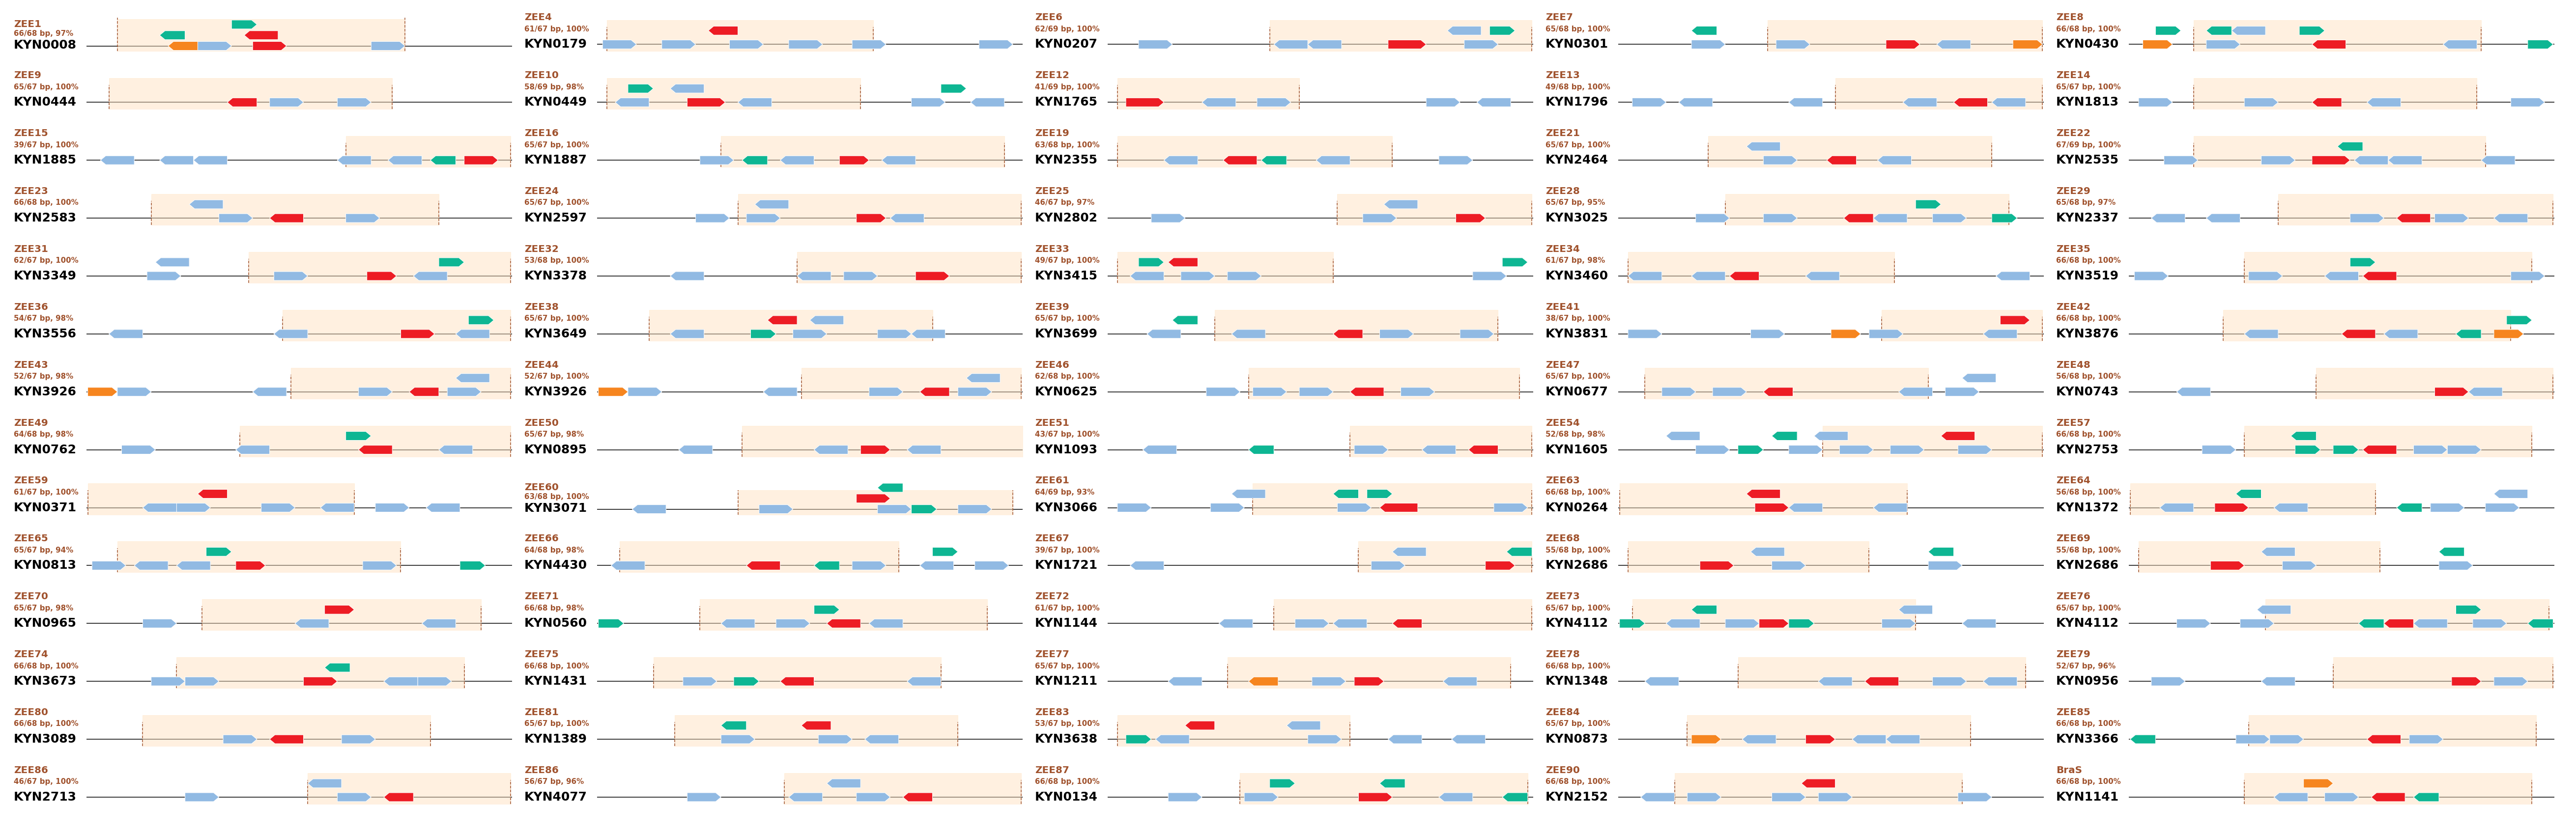
\includegraphics[scale=0.12]{3_figures-and-files/Fig1_ZEE-Comparison.png}
        \caption[The majority of ZEE sequences can be found in the KYN library]{\textbf{The majority of ZEE sequences can be found in the KYN library.} 
        As determined by Magic-BLAST, a total of 69/90 ZEE elements were found to overlap with members of the KYN library. Each diagram represented in the figure represents a schematic of the KYN enhancer, where the highlighted region represents the overlapping ZEE element that was detected by Magic-BLAST. The number of bases that aligned, along with the percentage alignment is also indicated. The colored binding sites represent the order, orientation, and spacing of Zic (red), ETS (blue), Bra (green), and FoxA (orange).}
        \label{fig:1 zee comparison}
    \end{figure}
\end{landscape}

\begin{figure}[h]
    \centering
    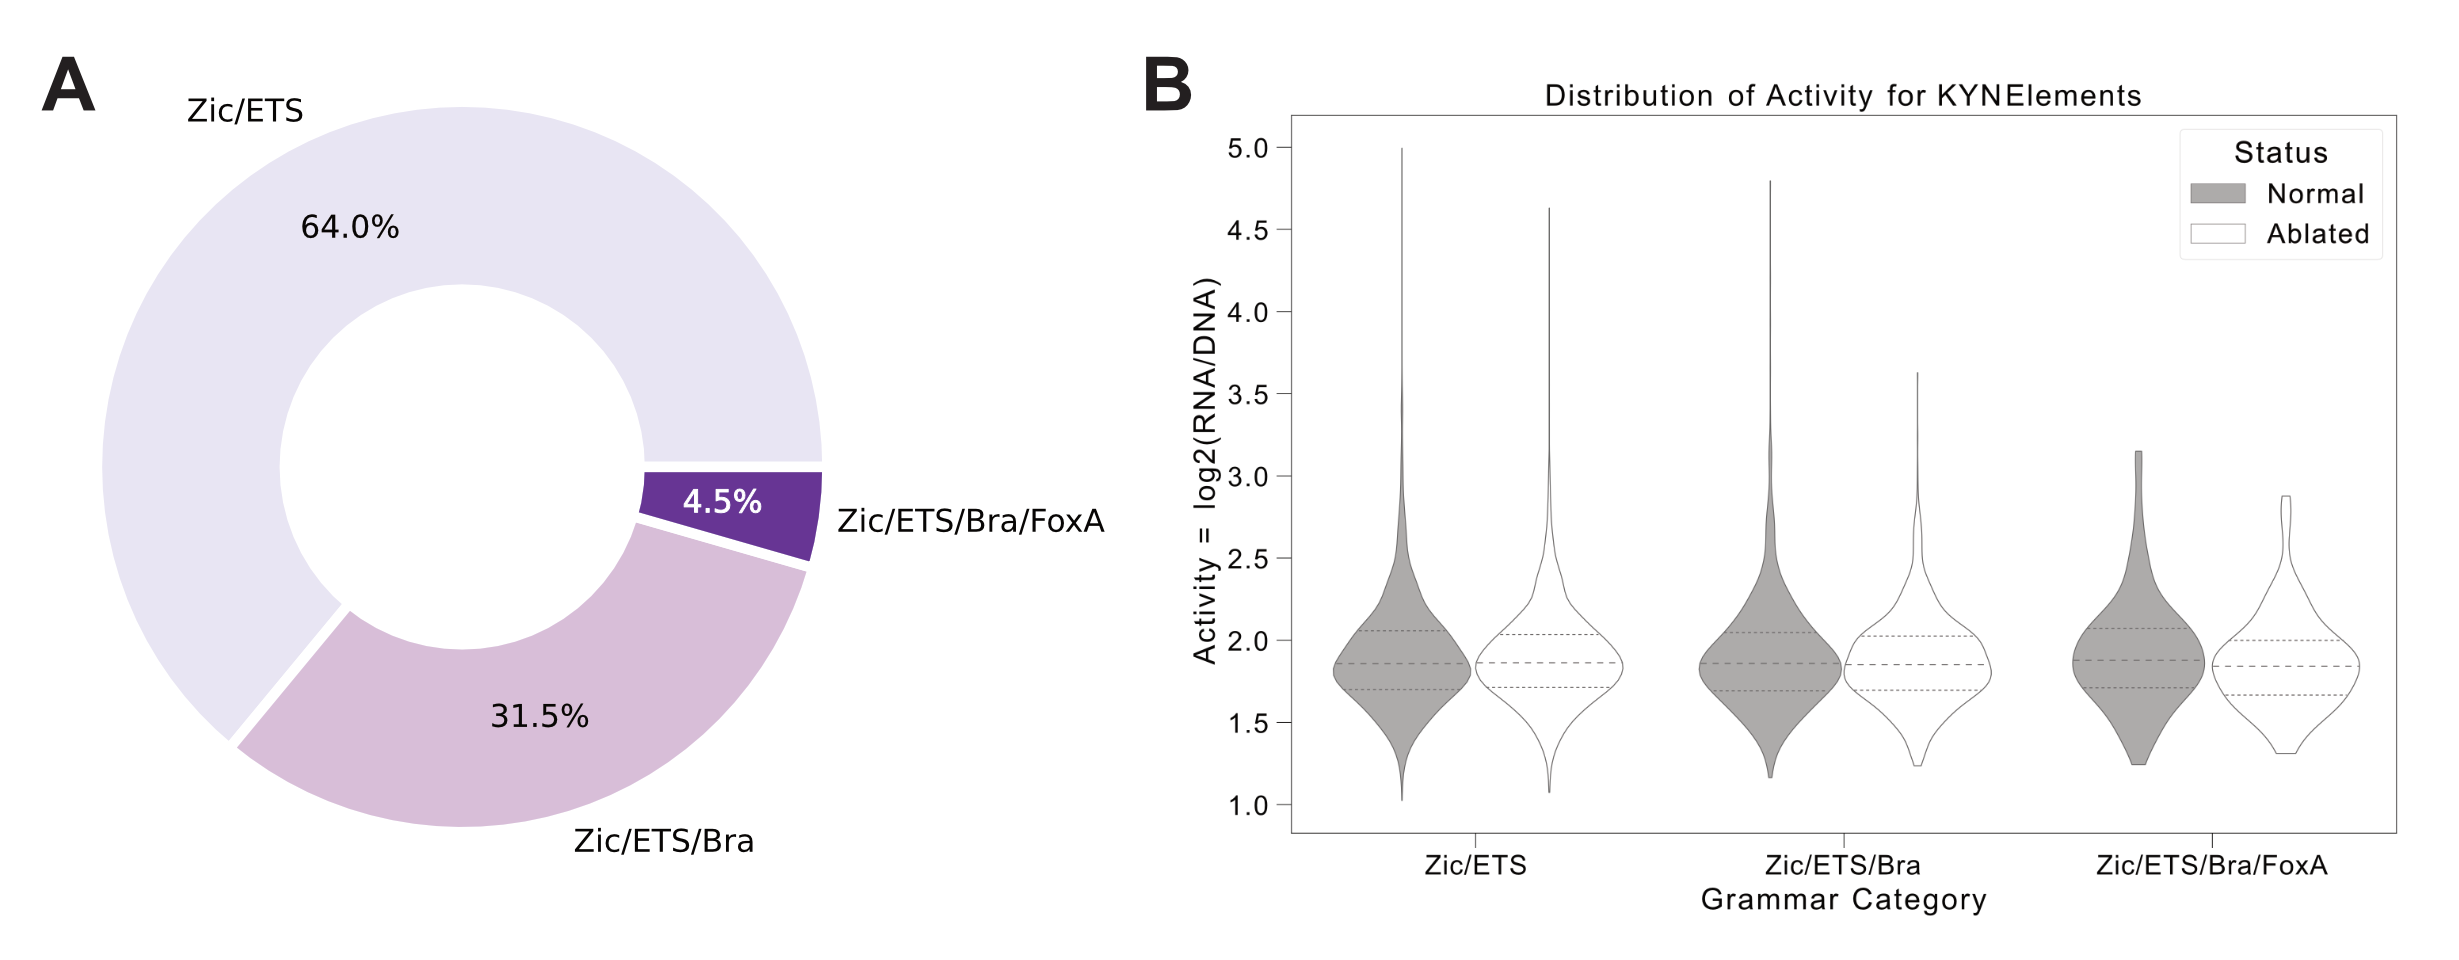
\includegraphics[scale=0.75]{3_figures-and-files/Fig2_Library-Information.png}
    \caption[ZEE Library Contents and Expression]{\textbf{ZEE Library Contents and Expression.} 
    \textbf{A.} The distribution of all 4,344 KYN elements across the Zic/ETS (pale lilac), Zic/ETS/Bra (pale magenta), and Zic/ETS/Bra/FoxA (violet) grammar categories. \textbf{B.} Violin plot showing the distribution of enhancer activity for the KYN library screen split across the Zic/ETS, Zic/ETS/Bra, and Zic/ETS/Bra/FoxA grammar categories. The grammar categories are also separated by the members of the KYN library that are "normal" (grey) or "ablated" (white). The lines in the violin plot represent the 25th, 50th, and 75th percentiles.}
    \label{fig:2 zee library}
\end{figure}

\subsection{Evaluating KYN genomic elements for enhancer activity in developing whole \textit{Ciona} embryos}

Next, we wanted to determine which KYN elements were functional by conducting an enhancer screen. We synthesized all 4,434 KYN elements upstream of a minimal promoter (bpFog) and a transcribable barcode. In addition to the ZEE elements that drove notochord expression in the previous study (Chapter \ref{chap:Diverse logics encode notochord enhancers}) \cite{song2022}, we wanted to evaluate how centering the Zic site within the sequence would impact expression. Thus, we took the sequences for the ZEE element with the highest enhancer activity, ZEE1 or LRIG1/2/3, and BraS, and centered the Zic site based on the sequence present in the updated \textit{Ciona} genome. Finally, we wanted to test the necessity of Zic and ETS for a given KYN element. To do this, we ablated the core of the Zic (\verb|GCWG| to \verb|GAWG|) and the core of the ETS (\verb|GGAW| to \verb|GCAW|) binding sites for each of the KYN elements and then included these sequences within the library for a total of 8,868 KYN elements. 

Ultimately, our enhancer screen ended up including 8,872 sequences, as we had some dropouts that were not present in the final massively-parallel reporter assay (MPRA). Each enhancer sequence was associated with, on average, 88 barcodes, where each barcode represents a specific measurement of enhancer activity. We then electroporated the enhancer library into fertilized \textit{Ciona} eggs. We collected embryos at the late gastrula stage (5.5 hours post fertilization, hpf), as this stage is where notochord cells are developing, and both Zic and ETS are expressed \cite{dykes2018,matsumoto2007a,song2022}. At this time point, we isolated both the mRNA and plasmid DNA and then sequenced the mRNA and DNA barcodes present. 

First, we filtered the data on if there was at least one mRNA or DNA barcode present for a given enhancer and if the Zic/ETS-ablated form of the enhancer was also present within the data. Next, we calculated an activity score for each KYN element. We first calculated the reads per million (RPM) for each mRNA and DNA barcode, then averaged the RPM across the mRNA and DNA barcodes associated with a given KYN element. To normalize the enhancer activity to differences in the amount of plasmid electroporated into each embryo, we took the $log_2$ of the average enhancer activity—mRNA RPM—divided by the average plasmid present—DNA RPM—for the same enhancer (Figure \ref{fig:2 zee library}B). We then filtered out enhancers in each replicate that were lower than two standard deviations lower than the mean $log_2$ value, as well as filtered out enhancers that were higher than the 99th percentile of standard deviation of $log_2$ values. In total, our library had 83.0\% of our expected sequences present (7,360/8,872 KYN sequences), including 85.7\% of the sequences that overlapped with the ZEE library (60/70 ZEE elements with successful KYN hits). The lowest and highest activity scores calculated were 1.02 and 4.99, respectively. In the following section, we discuss our identification of active enhancer elements within the KYN library.

\subsection{Several active KYN enhancers are proximal to genes implicated in the notochord and nervous system}

In our enhancer screen, we were interested in identifying enhancers that would decrease in expression upon ablation of the Zic and ETS binding sites to ensure the importance of these sites in conferring activity in our \textit{Ciona} embryos. We first filtered for functional enhancers by filtering for non-ablated regions with an activity score greater than or equal to the 90th percentile of the mean activity score or an activity score of 2.26. The 90th percentile was selected as an arbitrary cutoff that also acted as the most stringent. Next, we divided this group into three subsets based on the binding sites that were present: Zic/ETS, Zic/ETS/Bra, or Zic/ETS/Bra/FoxA. To determine enhancers whose activity depended on Zic and ETS, we searched for enhancers that had ablated counterparts with an expression below the 90th percentile cutoff. In total, we identified 438 active regions containing Zic and ETS, 204 active regions containing Zic, ETS, and Bra, and 29 active regions containing Zic, ETS, Bra, and FoxA that were dependent on Zic and ETS. To identify the top candidates from each category to evaluate further, we calculated the difference in enhancer activity between the “normal” and “ablated” sequences and sorted enhancers by this value. We then determined proximal genes by expanding approximately 5 kb on either edge of the sequence and annotating genes within this expanded window as proximal to our region of interest. The top five candidates within each category can be found in Table \ref{tab:top kyn elements across grammars}.

Upon looking over the top candidates, we see the largest differences between normal and their ablated variants in the grouping containing Zic and ETS and the grouping containing Zic, ETS, and Bra, whereas we see almost minimal difference between the normal and ablated variants in the grouping containing Zic, ETS, Bra, and FoxA. When reviewing the top five candidates from each grouping of TFBSs, we were surprised to find multiple genes implicated in nervous system disorders, especially regarding brain-associated conditions (e.g., spinocerebellar ataxia), such as \textit{RGS8}, \textit{RGS4}, \textit{SYS1}, \textit{ALDH4A1}, \textit{WARS2}, \textit{ITPR1}, \textit{XRN2}, \textit{KCNQ3}, and \textit{OTX1}. Several genes were also implicated in skeletal and bone-related disorders, such as \textit{HOXD3}, \textit{DYNLT2B}, and \textit{FLG}. While we have put these enhancers into these three groups, we do not know if the Bra and FoxA sites are contributing to their activity. However, we do know that these enhancers are dependent on Zic and ETS, two transcription factors critical in neural and notochord development. Ultimately, more exploration is needed to discern if these regions are truly functional within the \textit{Ciona} notochord through imaging studies, but their primary association with homologous human genes is promising. Additionally, more work is needed to ascertain if known disease-associated SNPs fall within regions containing potential notochord enhancer grammars consisting of Zic, ETS, Bra, and FoxA binding sites. 

\begin{small}
    \begin{landscape} % this table is long, so it'll be multi-page landscape
        \begin{longtable}{l l p{.18\textwidth} p{.15\textwidth} p{.15\textwidth} p{.15\textwidth} p{.2\textwidth}}
            % Define the table title in the table of contents
            \caption{Top five KYN elements across grammatical categories} 
            \label{tab:top kyn elements across grammars}
            \\ \hline 

            % Define the table columns for the first and all subsequent pages
            \multicolumn{1}{l}{\textbf{GRAMMAR}} & \multicolumn{1}{l}{\textbf{KYN ID}} & \multicolumn{1}{l}{\textbf{LOCATION}} & \multicolumn{1}{l}{\textbf{ACTIVITY(N)}} & \multicolumn{1}{l}{\textbf{ACTIVITY(A)}} & \multicolumn{1}{l}{\textbf{ACTIVITY(N-A)}} & \multicolumn{1}{l}{\textbf{PROXIMAL GENES}} \\ \hline \endfirsthead

            \multicolumn{7}{l}%
            {{\textbf{\tablename\ \thetable{}.} Top five KYN elements across grammatical categories, \textit{continued from previous page}}} \\
            \hline 
            \multicolumn{1}{l}{\textbf{GRAMMAR}} & \multicolumn{1}{l}{\textbf{KYN ID}} & \multicolumn{1}{l}{\textbf{LOCATION}} & \multicolumn{1}{l}{\textbf{ACTIVITY(N)}} & \multicolumn{1}{l}{\textbf{ACTIVITY(A)}} & \multicolumn{1}{l}{\textbf{ACTIVITY(N-A)}} & \multicolumn{1}{l}{\textbf{PROXIMAL GENES}} \\
            \hline\hline \endhead

            % Define the table footer for the first and all subsequent pages
            \hline \multicolumn{7}{r}{\textit{Continued on next page}} \\ \hline \endfoot
            \hline \endlastfoot
            
            % Start table content

            %%%%% %%%%% %%%%% %%%%% %%%%% %%%%% %%%%% %%%%% %%%%% %%%%% %%%%% %%%%%
            Zic/ETS & KYN4389 & chr9:2616602-2616702 & 4.57 & 1.98 & 2.59 & \textit{POM121L2}, \textit{RGS8}, \textit{RGS4} \\
            Zic/ETS & KYN4390 & chr9:2616623-2616723 & 4.26 & 1.97 & 2.29 & \textit{POM121L2}, \textit{RGS8}, \textit{RGS4} \\
            Zic/ETS & KYN1765 & chr2:2253506-2253606 & 3.38 & 1.58 & 1.79 & \textit{ERCC5}, \textit{SYS1}, \textit{ESD} \\
            Zic/ETS & KYN0616 & chr10:1184720-1184820 & 3.75 & 1.99 & 1.76 & \textit{ALDH4A1}, \textit{CBL} \\
            Zic/ETS & KYN0516 & chr1:14250867-14250967 & 3.61 & 1.95 & 1.66 & \textit{HOXD3}, \textit{DYNLT2B} \\
            
            Zic/ETS/Bra & KYN2946 & chr6:381260-381360 & 4.79 & 1.71 & 3.08 & \textit{WARS2} \\
            Zic/ETS/Bra & KYN3554 & chr8:5563238-5563338 & 2.79 & 1.33 & 1.46 & \textit{ITPR1} \\
            Zic/ETS/Bra & KYN0942 & chr11:2883954-2884054 & 2.74 & 1.37 & 1.36 & \textit{YME1L1} \\
            Zic/ETS/Bra & KYN2661 & chr4:6611261-6611361 & 3.12 & 1.82 & 1.31 & \textit{SEMA6A}, \textit{ADAMTSL1} \\
            Zic/ETS/Bra & KYN1322 & chr12:6286408-6286508 & 2.87 & 1.58 & 1.29 & \textit{PTPRF}, \textit{PTPRQ}, \textit{DNAJA1} \\

            Zic/ETS/Bra/FoxA & KYN4030 & UAContig6:165904-166004 & 3.12 & 2.03 & 1.08 & \textit{FLG}, \textit{GIN1}, \textit{XRN2}, \textit{HUS1B}, \textit{KCNQ3} \\
            Zic/ETS/Bra/FoxA & KYN3090 & chr7:319156-319256 & 2.58 & 1.57 & 1.00 & \textit{ELAC2} \\
            Zic/ETS/Bra/FoxA & KYN4335 & chr4:4509497-4509597 & 2.90 & 1.94 & 0.96 & \textit{OTX1}, \textit{CETN2} \\
            Zic/ETS/Bra/FoxA & KYN1404 & chr13:639638-639738 & 2.72 & 1.77 & 0.95 & \textit{PIK3AP1}, \textit{KCNJ5} \\
            Zic/ETS/Bra/FoxA & KYN4230 & chr10:4824445-4824545 & 2.49 & 1.59 & 0.90 & \textit{ANGPT2} \\
        \end{longtable}
    \end{landscape}
\end{small}

\subsection{Identifying genomic regions containing Zic and ETS binding sites in other species}

In hopes of finding additional regions for us to evaluate in the future, we applied our methodology to gather KYN regions from \textit{Ciona} to other vertebrate species. We also searched the \textit{Ciona savigni} for regions containing Zic and ETS binding sites to compare against \textit{Ciona intestinalis type A}. The number of regions obtained in this approach can be found in Table \ref{tab:genome search vertebrate numbers}. As expected, with an increase in the genome size, we see an increase in the number of sites with Zic and ETS binding sites. More exploration is needed to evaluate where these regions fall in relation to notochord and neural-associated genes and if the grammar between our various transcription factors of interest is comparable across members of Chordata. 

\begin{small}
    \begin{table}[ht]
        \centering
        \caption{Number of regions containing Zic and ETS found across other species} 
        \begin{tabular}{|l|l|l|l|}
            \hline
            % Define the table columns for the first and all subsequent pages
            \textbf{NAME} & \textbf{SCIENTIFIC NAME} & \textbf{GENOME ASSEMBLY} & \textbf{REGIONS} \\ \hline 
            
            % Start table content

            %%%%% %%%%% %%%%% %%%%% %%%%% %%%%% %%%%% %%%%% %%%%% %%%%% %%%%% %%%%%
            Solitary sea squirt & \textit{Ciona savignyi} & CSAV2\footnote{\href{http://mendel.stanford.edu/SidowLab/ciona.html}{http://mendel.stanford.edu/SidowLab/ciona.html}} \cite{hill2008} & 8,061\\
            Chicken & \textit{Gallus gallus} & galGal6\footnote{\href{http://genome.ucsc.edu/cgi-bin/hgGateway?db=galGal6}{http://genome.ucsc.edu/cgi-bin/hgGateway?db=galGal6}} & 121,913\\
            Zebrafish & \textit{Danio rerio} & danRer11\footnote{\href{http://genome.ucsc.edu/cgi-bin/hgGateway?db=danRer11}{http://genome.ucsc.edu/cgi-bin/hgGateway?db=danRer11}} & 170,972\\
            Mouse & \textit{Mus musculus} & mm10\footnote{\href{http://genome.ucsc.edu/cgi-bin/hgGateway?db=mm10}{http://genome.ucsc.edu/cgi-bin/hgGateway?db=mm10}} & 182,575\\
            Human & \textit{Homo sapiens} & hg38\footnote{\href{http://genome.ucsc.edu/cgi-bin/hgGateway?db=hg38}{http://genome.ucsc.edu/cgi-bin/hgGateway?db=hg38}} & 179,501\\
            \hline
        \end{tabular}
        \label{tab:genome search vertebrate numbers}
    \end{table}
\end{small}

\subsection{Developing a proof-of-concept software package for clusters of binding sites within genomes}

Finding our preliminary exploration into active enhancers promising, we wanted to develop a tool that could translate our genomic searches in \textit{Ciona} and other vertebrates to other organisms that we did not feature within this study. We then developed a method to look for clusters of binding sites within genomes in Python called Entire Genome seArches for Grammars of Enhancers (EnGAGE, \href{https://github.com/farleylab/engage-tools}{\texttt{engage-tools} GitHub Repository Link}). 

EnGAGE is a proof-of-concept Python package to search for clusters of TFBS motifs of choice within an input reference genome using regular expression definitions of binding sites. Using EnGAGE, users can define a \verb|Cluster| parent class object to which they can add various child class \verb|TF| objects. These \verb|TF| objects represent individual transcription factor binding motifs in. After the parameters have been set, the user can use the \verb|find_motif_cluster()| method to search through any genome of interest for locations of particular clusters for further exploration. As more information is learned about enhancers, additional constraints on TFBS syntax and affinity can be added to the \verb|Cluster| object to search for functional grammars.

%%%%%%%%%%%%%%%%%%%%%%%%%%%%%%%%%%%%%%%%%%%%%%%%%%%%%%%%%%%%%%%%%%%%%%%%%%%%%%%%
\section{Discussion}
%%%%%%%%%%%%%%%%%%%%%%%%%%%%%%%%%%%%%%%%%%%%%%%%%%%%%%%%%%%%%%%%%%%%%%%%%%%%%%%%

The marine chordate \textit{Ciona} is easily amenable to high-throughput enhancer studies, making it a valuable model system for studying functional genomics. The \textit{Ciona} genomic reference sequence was recently reassembled based on modern sequencing techniques, providing dramatic improvements over the previous reference genome from the early 2000s \cite{satou2019,dehal2002}. In this work, we sought to lay the groundwork for future studies to understand the regulatory logic of notochord enhancers we discovered in a previous study of Zic, ETS, FoxA, and Brachyury binding sites (Chapter \ref{chap:Diverse logics encode notochord enhancers}) \cite{song2022}. While we found a total of 4,344 elements in the \textit{Ciona} genome containing at least one Zic site and two ETS sites, testing these elements in an MPRA revealed that only 15.4\% of these sites (671/4,344 regions) were active \textit{and} dependent on Zic and ETS. Further study of this enhancer library will likely identify novel notochord enhancers and help us better understand how Zic and ETS encode notochord development through particular grammatical constraints. 

\subsection{Differences between the ZEE library and KYN library}

After searching for new elements in the updated \textit{Ciona} genome to formulate the KYN library, we wanted to evaluate if there was an overlap between these elements and our previous study of the ZEE elements (Chapter \ref{chap:Diverse logics encode notochord enhancers}) \cite{song2022}. While we could corroborate the majority of ZEE elements within the updated KYN library using Magic-BLAST \cite{boratyn2019}, the amount of overlap varied, and some sequences had perfect alignment but less than 50 bp of overlapping sequence (e.g., ZEE12, ZEE13, ZEE15, and ZEE33) (Figure \ref{fig:1 zee comparison}). Additionally, the sizes of the regions between the ZEE library and KYN library varied. Regions tested in the ZEE library were approximately 69 bp in length (Chapter \ref{chap:Diverse logics encode notochord enhancers}) \cite{song2022}, whereas regions tested in the KYN library were fixed at 100 bp. The additional length of the KYN library has the potential to introduce additional sequence elements that would cause discordance between the ZEE and KYN library results. Indeed, when we evaluate the expression between ZEE elements and KYN elements, there are elements from the ZEE library with notochord expression that are only moderately active in the KYN library and vice versa. 

\subsection{Further exploration is needed to understand active KYN elements}

Without much overlap between the sequences of the ZEE library and KYN library (Figure \ref{fig:1 zee comparison}), it was difficult to determine the threshold for determining active enhancers within our study. Thus, we set a stringent threshold and strict filtering criteria to label active enhancers within our study; all elements within our study were required to have an enhancer activity greater than the 90th percentile of overall activity. Overall, this allowed us to identify potentially interesting targets for future study (Table \ref{tab:top kyn elements across grammars}). 

Unfortunately, while the ablation studies help us understand the necessity of Zic and ETS binding sites present within the KYN elements, they do not allow us to ascertain the importance of other binding sites, such as Bra and FoxA. Indeed, some of the elements in which Zic and ETS binding site ablation leads to similar or higher levels of enhancer activity compared to their original sequence may be dependent on the Bra or FoxA sites or other TFBSs that we have not yet identified (\textit{not featured in this study}). Thus, more exploration is needed to image these elements, conduct follow-up experiments to dissect these sequences and determine proper thresholds for future work.

%%%%%%%%%%%%%%%%%%%%%%%%%%%%%%%%%%%%%%%%%%%%%%%%%%%%%%%%%%%%%%%%%%%%%%%%%%%%%%%%
\section{Materials and Methods}
%%%%%%%%%%%%%%%%%%%%%%%%%%%%%%%%%%%%%%%%%%%%%%%%%%%%%%%%%%%%%%%%%%%%%%%%%%%%%%%%

\subsection{\textit{Ciona intestinalis} dechorionated, \textit{in vitro} fertilization, and electroporation}
Adult \textit{\textit{Ciona} intestinalis type A}, also known as \textit{\textit{Ciona} robusta}, were obtained from M-Rep and were maintained under constant illumination in seawater (obtained from Reliant Aquariums) at $18^\circ$C. \textit{Ciona} are hermaphroditic, therefore, there is only one possible sex for individuals. Age or developmental stage of the embryos studied is indicated in the main text. Methods for dechorionated, \textit{in vitro} fertilization, and electroporation were performed as described previously in Farley et al., 2016 \cite{farley2016}.

\subsection{Identification of KYN putative notochord enhancers and conducting vertebrate genome searches for elements containing Zic and ETS binding sites}
We identified elements in the updated \textit{Ciona} genome by first identifying clusters of Zic and ETS sites across each chromosome. We used the following sites and their corresponding reverse complement sequence in our search for Zic binding sites: \verb|CAGCTGTG| (Zic1/2/3), \verb|CCGCAGT| (Zic7/3/1), \verb|CCGCAGTC| (Zic6), \verb|CCCGCTGTG| (Zic1), \verb|CCAGCTGTG| (Zic3), \verb|CCGCTGTG| (Zic2/ZicC), and \verb|CCCGCAGTC| (Zic5) as these have been identified as functional in previous studies (Matsumoto et al., 2007a; Yagi et al., 2004) \cite{matsumoto2007a,yagi2004}. Methods for obtaining genomic regions to include in the KYN library and the vertebrate genomes included in Table \ref{tab:genome search vertebrate numbers} can be found in Supplementary Figure \ref{fig:supplement kyn library search}.

\subsection{Construction of the KYN enhancer library}
The genomic regions were ordered from Agilent Technologies with adapters containing BseRI sites. This was cloned into the custom-designed SEL-Seq (Synthetic Enhancer Library-Sequencing) vector using type II restriction enzyme BseRI. After cloning, the library was transformed into bacteria (MegaX DHB10 electrocompetent cells), and the culture was grown up until an OD of 1 was reached. DNA was extracted using the Macherey-Nagel Nucleobond Xtra Midi kit. A 30 bp barcode with adapters containing Esp3I sites was cloned into this library using type II restriction enzyme Esp3I. The library was transformed into bacteria (MegaX DHB10 electrocompetent cells) and grown up until an OD of 2 was reached. The DNA library was extracted from the bacteria using the Macherey-Nagel Nucleobond Xtra Midi kit. 

\subsubsection{Enhancer to barcode tag assignment \& enhancer dictionary analysis}
We constructed a dictionary of unique barcode tag-enhancer pairs by not allowing for any mismatches in the 100 bp enhancers in our library and by not allowing barcode tag-enhancer pairs to have a read count of fewer than 25 reads. Additionally, we required all barcode tags to be 29 bp or 30 bp in length. If more than one barcode tag was associated with a single enhancer, we included all associated barcode tags that met the aforementioned barcode length and read count requirements. Within our dictionary, there were 40 barcode tags that were matched to multiple enhancers and thus discarded from the final dictionary. In total, the dictionary contained 748,258 total barcode tag-enhancer associations and 8,460 total enhancers that were uniquely mapped to one or more barcode tags. The median and mean number of barcode tags associated with a single enhancer were 76 and 88, respectively.  

\subsection{Conducting the KYN MPRA screen}
50 $\mu$g of the KYN library was electroporated into ~5,000 fertilized eggs. Embryos developed until 5 hours and 30 minutes at $22^\circ$C. Embryos put into TriZol, and RNA was extracted following the manufacturer's instructions (Life Technologies). The RNA was DNase treated using Turbo DNaseI from Ambion following standard instructions. Poly-A selection was used to obtain only mRNA using poly-A biotinylated beads as per instructions (Dyna-beads, Life technologies). The mRNA was used in an RT reaction that was specifically selected for the barcoded mRNA (Transcriptor High Fidelity, Roche). The RT product was PCR amplified and size selected using Agencourt AMPure beads (Beckman Coulter), then checked for quality and size on the 2100 Bioanalyzer (Agilent) and sent for sequencing on the NovaSeq S4 PE100 mode (Illumina). Three biological replicates were sent for sequencing. 

The DNA was extracted by mixing the phenol-chloroform and interphase of TriZol extraction with 500 $\mu$L of Back Extraction Buffer (4 M guanidine thiocyanate, 50 mM sodium citrate, and 1 M Tris-base). DNA was treated with RnaseA (Thermo Fisher). DNA was cleaned up with phenol:chloroform:isoamyl alcohol (25:24:1) (Life Technologies). The DNA was PCR amplified and size selected using Agencourt AMPure beads (Beckman Coulter), then checked for quality and size on the 2100 Bioanalyzer (Agilent) and sent for sequencing on the NovaSeq S4 PE100 mode (Illumina). Three biological replicates were sent for sequencing.

\subsubsection{SEL-Seq data analysis}
For the whole embryo library, we sequenced barcode tags from the DNA and RNA libraries on the Illumina HiSeq 4000. Reads that perfectly matched barcode tags in our barcode tag-enhancer dictionary were included in the subsequent analysis. We extracted all of the read sequences from the sequencing libraries and collapsed them based on unique sequences, tabulating the number of times a unique sequence appears in the library. Next, we perform preliminary filtering on the unique sequences, filtering out sequences that (i) have \verb|N|’s present, (ii) are missing the GFP sequence after our expected location of the barcode tag, (iii) contain a barcode that is not an exact match to our enhancer-barcode tag dictionary, (iv) did not meet the minimum read cutoff of 25 reads. All DNA and RNA libraries were processed separately for the preliminary filtering step. 

Prior to normalizing our data into RPM, we first filtered out all enhancers that did not have their ablated pair present within the sample. We then filtered our data further to only include the set of barcode tags and enhancers that appear in DNA across all replicates. We then consolidated the expression for each enhancer by taking the average RPM value across barcode tags. To determine if an enhancer was active, we calculated an “enhancer activity score.” This score is calculated by averaging the $log_2({\frac{RNA}{DNA}})$ value across a given enhancer’s biological replicates. 

%%%%%%%%%%%%%%%%%%%%%%%%%%%%%%%%%%%%%%%%%%%%%%%%%%%%%%%%%%%%%%%%%%%%%%%%%%%%%%%%
\section{Acknowledgements}
%%%%%%%%%%%%%%%%%%%%%%%%%%%%%%%%%%%%%%%%%%%%%%%%%%%%%%%%%%%%%%%%%%%%%%%%%%%%%%%%
I would like to thank the following individuals that made this work possible: Benjamin P. Song, Jessica L. Grudzien, Sophia H. Le, Joe J. Solvason, and Emma K. Farley. I would also like to thank the Farley Lab, Hannah Carter, and the Carter Lab--especially Adam Klie--for helpful discussions during the analysis and visualizations of the data included in this chapter. I would also like to thank the team at the UCSD IGM Genomics Center for their assistance with sequencing. 

%%%%%%%%%%%%%%%%%%%%%%%%%%%%%%%%%%%%%%%%%%%%%%%%%%%%%%%%%%%%%%%%%%%%%%%%%%%%%%%%
\section{Footnotes}
%%%%%%%%%%%%%%%%%%%%%%%%%%%%%%%%%%%%%%%%%%%%%%%%%%%%%%%%%%%%%%%%%%%%%%%%%%%%%%%%

\subsection{Author contributions}
E.K.F., B.P.S., M.F.R, designed experiments. B.P.S., J.L.G., and S.H.L. conducted experiments. M.F.R. conducted bioinformatic analyses. M.F.R. and J.J.S. were involved in the software development of EnGAGE. M.F.R. wrote the chapter. E.K.F., M.F.R., and B.P.S. were involved in editing the chapter. 

\subsection{Funding}
M.F.R. was supported by NIH T32 GM008666. B.P.S. was supported by NIH T32 GM133351. J.J.S. was supported by NIH T32GM127235. E.K.F., B.P.S., M.F.R., J.L.G., S.H.L., and J.J.S. were supported by NIH DP2HG010013.

\subsection{Data availability}
Further information and requests for resources and reagents should be directed to and will be fulfilled by the lead contact, Emma K. Farley (efarley@ucsd.edu), upon request. All plasmids generated in this study and KYN screen sequencing data will be deposited to Addgene and GEO, respectively, when a publication is made available. All original code has been deposited to GitHub (\href{https://github.com/farleylab/Expanded-Notochord-Logics-Study}{https://github.com/farleylab/Expanded-Notochord-Logics-Study}) and is publicly available. The code for the proof-of-concept tool, EnGAGE, has also been deposited to GitHub (\href{https://github.com/farleylab/engage-tools}{https://github.com/farleylab/engage-tools}) and is publicly available. Any additional information or data required to recapitulate the study reported in this chapter is available upon request.

\subsection{Declaration of interests}
The authors declare no competing interests.
